\chapter{Discovering Trends of Drug Abuse from Social Media Data}
\label{AB_chapter}
\section{Introduction}
Nonmedical use of prescription medications/drugs (NMUPD), 
particularly prescription analgesic opioid abuse, 
is a grave threat to the nation's health. 
In fact, the U.S. Centers for Disease Control and Prevention 
recorded a record number of drug overdose deaths in 2014, 
headlined by a nearly fourfold increase in prescription 
opioid-related drug mortality since 1999, 
further coupled by increased heroin injection drug use 
associated with NMUPD behavior 
(Centers for Disease Control and Prevention (CDC), 2011;  
Centers for Disease Control and Prevention (CDC), 2013; 
\cite{compton2016relationship}, \cite{rudd2016increases}). 
As this public health crisis continues to gain public attention, 
so does the need for better data identifying underlining 
NMUPD behaviors, trends, and risk factors in order to optimize 
efforts at improving access to treatment, 
preventing overdose, and ensuring community interventions are effective. 
Currently, existing NMUPD data is largely derived from national 
population-based surveys that measure the prevalence estimates, 
attitudes, and associated trends of various forms of substance abuse (including NMUPD) 
and rely upon respondents to self-report their past drug use 
behaviors via face-to-face interviews or self-administered questionnaires 
(\cite{katsuki2015establishing, schepis2016trends}). 
These survey-based instruments are critical in identifying 
generalizable trends of prescription drug abuse behavior in a 
national population, assessing changes in what classes of prescription drugs 
are becoming popular targets of abuse, and aid in the development of 
targeted interventions and policy to address risk and protective factors common to 
NMUPD \cite{han2015nonmedical}.

However, even powerful nationally representative surveys, 
such as the National Survey on Drug Use and Health and the Monitoring 
the Future survey (which focuses on students and young adults), 
have certain inherent limitations \cite{schepis2016trends,mccabe2012co,mccabe2013leftover}. 
Most evidently, they largely rely on respondents to self-report and recall recent 
and past drug abuse behavior, a methodology that can be subject to 
recall bias \cite{harrison1997validity}. Further, results from these 
surveys generally take time to compile after data collection is completed, 
with trends reported from these observations possibly changing by the time survey results are 
reported \cite{katsuki2015establishing}.

Hence, alternative methods for conducting surveillance of NMUPD 
behavior are needed to augment findings from national substance abuse 
surveys, including leveraging the power of ``big data" analysis and social media 
platforms that are now heavily populated by a wide demographic of the substance 
using population, a practice now popularized as ``digital epidemiology" or 
``infoveillance \cite{salathe2012digital}."

Despite, growing opportunities in a growing digitized social sphere, 
the massive size of these datasets and accompanying challenges of filtering, 
processing and analyzing the data in a meaningful way, has left the field ripe for 
innovation and improvement, particularly through cross-disciplinary research 
collaborations. In response, this study advances prior studies that have examined 
the linkages between Twitter and NMUPD and introduces a new methodology 
leveraging recent developments in computer science in order to gain a 
“bigger” picture of national NMUPD trends. Previous studies have used 
methodologies focusing on content analysis and human coding/annotation 
using keyword searches, identifying subsets of Twitter NMUPD-related 
social circles, and analyzing a random sample of filtered tweets 
\cite{hanson2013tweaking,hanson2013exploration,katsuki2015establishing,shutler2015drug}.

In this study, we similarly conducted surveillance of the popular 
microblogging site Twitter (which now commands 310 million active users) 
filtered for content posted by users that specifically mentioned 
prescription analgesic opioid drugs. However, because of the massive amount 
of data required to be analyzed and given that content on Twitter is not 
curated for information specifically relevant to NMUPD, Twitter datasets 
often contain a high number of tweets that are non-relevant to NMUPD 
(i.e. noise) compared to content that actually describes NMUPD-related 
behavior (i.e. signal content). This condition necessitates a methodology 
that can iteratively filter tweets to eliminate noise and only 
retain tweets relevant to NMUPD behavior similar to those used in 
other studies examining other important public health issues 
\cite{chen2014flu,prier2011identifying}. Concomitantly, by 
filtering only for NMUPD relevant content, this methodology 
subsequently analyzes the tweets to discover and identify the 
different underlying latent themes that exist in the entire dataset. 
Hence, our study's methodology differs from prior studies because 
it can be used to highly automate filtering and coding of an 
extremely large dataset of tweets and simultaneously 
identify key NMUPD themes that are occurring in the entire 
Twittersphere in order to better inform researchers and 
the public about changes in the prescription opioid epidemic.


\section{Methods}
\subsection{Overall aims}
This study was conducted in two distinct phases: 
data collection and data analysis. The goal of this study included 
two distinct aims related to data processing and analysis to identify 
risk behaviors associated with NMUPD as reported in content generated by Twitter users. 
The first aim was to increase the signal to noise ratio in 
the dataset of all tweets analyzed and weed out tweets that are not 
relevant to NMUPD behavior. The second involved identifying themes and
patterns from the large corpus of Tweets in order to gain a broader 
understanding of NMUPD behaviors for a larger Twitter user population that 
included more than 11 million tweets collected during a six-month period. 
In order to handle a dataset of this magnitude it is necessary to develop 
methodologies to be as automated as possible and limit the amount of human coding, 
in order to scale big data collection, surveillance and analysis. 
Section \ref{AB:data_collection} 
describes the data collection process used to generate large amounts of 
tweets on NMUPD from the Twitter Application Programming Interface (API) stream. 
Section \ref{AB:analysis_plan} describes the 
iterative methodology that was employed to 
increase the signal to noise ratio in the dataset, 
and to identify patterns and themes present in the data specific to analgesic opioid NMUPD.

\subsection{Data collection}
\label{AB:data_collection}
Twitter provides a public API that enables the collection 
of messages publicly posted by its users via its online platform. 
We used a data collection methodology involving cloud-based computing 
services offered by Amazon Web Services (AWS) and virtual computers via 
Amazon EC2 t2.micro instances set to filter and collect tweet 
objects containing specific NMUPD keywords.

Keywords included brand and international non-proprietary 
(e.g. generic) names (INN names) of commonly abused prescription 
analgesic opioid drugs. The data collection methodology used 
for this study has been previously described in detail in a prior 
published study (\cite{katsuki2015establishing}). 
INN names of prescription opioid drugs included: Percocet (acetaminophen/oxycodone),
OxyContin (oxycodone) and Oxycodone and were used in conjunction 
with the streaming API in order to track tweet objects that potentially 
contain at least one of these keywords. This generated a total of 
approximately 11M English-language tweets that were collected 
between the period of June and November 2015. A summary of the 
number of tweets collected for each drug is provided in Table \ref{table:drugs_summary}. 
Additionally, during the preprocessing of the data, 
any identifiable information (e.g. Twitter account names, etc.) 
was removed from prior to data analysis.

\begin{table}
\centering
\begin{tabular}{|c|c|c|}
\hline
Keywords &   \#-of-tweets & \% of English tweets \\
Percocet &  8,004,229  & 94.24 \\
OxyContin & 3,280,910  & 92.16 \\
Oxycodone  & 2,315,321 &  88.90 \\
\hline
\end{tabular}
\caption[Summary of the number of tweets collected.]{Summary of keywords used in 
conjunction with the Twitter 
Streaming API for data collection and the corresponding number of tweets collected.}
\label{table:drugs_summary}
\end{table}

\subsection{Analysis Plan}
\label{AB:analysis_plan}

In order to appropriately code, identify, and characterize large 
volumes of data collected from social media sites in the context 
of public health issues, the application of machine learning has 
become a critical strategy in digital surveillance. The need for 
the application of machine learning has been necessitated by the 
sheer enormity of the data used for analysis when generating data 
from public sources like the Twitter API. Machine learning, especially 
unsupervised machine learning models are efficient at automatically 
finding patterns in the data and summarizing the content of the 
text corpus. The algorithms are computationally efficient and results 
have the advantage of not being affected by potential human judgment bias.

In the machine learning literature, there exist models which, 
when given a text corpus, are able to identify the underlying latent 
patterns or themes or (more formally in the machine learning 
literature) topics present in the corpus. Such models are 
referred to as topic models owing to their ability to summarize 
the content of the corpus concisely in terms of a few distinct topics 
\cite{blei2003}. With the advent of Twitter and other microblogging 
sites as a potent source of textual data, a model called the 
Biterm Topic Model (BTM) was proposed specifically to detect 
themes and patterns in corpora of short-texts \cite{yan2013biterm}.

The methodology for our work is built by using 
BTM as the core for recognizing patterns in our corpus of tweets. 
BTM, when given a corpus of tweets as a parameter $k$ 
for the number of themes to be identified as inputs identifies $k$ 
underlying themes in the corpus. This is the learning phase of 
BTM. As the output of this phase, it produces a discrete 
probability distribution for all words for each theme. 
Ideally, this distribution would place large weights on 
the words that are most representative of that theme. 
Hence, a ranking of the top-10 words produced by 
BTM for each theme can be used as a summary 
representing all the themes present in the input corpus.

BTM also operates in what is called the inference phase. 
In this phase, BTM has the ability to decompose each tweet 
in terms of the themes identified in the learning phase. 
As the output of this phase, BTM produces a histogram for 
each tweet where each bin represents a theme discovered in 
the learning phase. The value in that bin represents how 
correlated the given tweet is to that particular theme. 
A tweet highly correlated to a particular theme will have, 
in its histogram representation, a large weight placed 
in the corresponding bin. The inference phase of BTM 
essentially enables us to retrieve the tweets most 
correlated to a particular theme.

First, the dataset was separated according to the keywords filtered in Table \ref{table:drugs_summary}. 
Once a subset of tweets corresponding to each drug was obtained, 
a two-step iterative process was employed. 
The first step involved detecting $k$ themes from the set of tweets 
corresponding to each drug using the learning phase of BTM. 
The second step involved manually identifying themes that produced false positive 
content; i.e., content irrelevant to NMUPD behavior and promotion. 
For this step, the top ranked words in each theme 
(produced in the first step) were analyzed in conjunction 
with the inclusion/exclusion rules laid out in Table \ref{table:inclusion_exclusion} 
to determine whether or not a theme was relevant to NMUPD behavior.

\begin{table}
\centering{c}
\begin{tabular}{|c|}
\hline
\pbox{20cm}{Contains INN or slang names identified by NIDA of a prescription drug subject to abuse.}\\
\pbox{20cm}{Mentions of other illicit drugs (e.g., heroin, cocaine, marijuana) and/or alcohol.}\\
\pbox{20cm}{Mentions of identified substance abuse risk behavior (e.g. overdose, injection, withdrawal).}\\
\pbox{20cm}{Contains adjectives related to prescription drug abuse behavior (e.g., popping).}\\
\hline
\end{tabular}
\caption[Inclusion exclusion rules for topics.]{Summary of rules applied to determine if a theme was relevant for inclusion in subsequent iterations.}
\label{table:inclusion_exclusion}
\end{table}

Prior studies that have utilized content analysis and human annotation 
in order to filter out tweets that are not explicitly related to 
individual NMUPD behavior (e.g. tweets containing news reports, 
automated feeds, tweets by commercial entities, illicit online sales, etc.) 
\cite{katsuki2015establishing,hanson2013tweaking,hanson2013exploration,shutler2015drug}
(Hanson et al., 2013a; Hanson et al., 2013b; Katsuki et al., 2015 ;  Shutler et al., 2015). 
We used a similar filtering scheme instead relying upon our machine 
learning BTM protocol to identify tweets that contained 
NMUPD-related behavior content of interest. Specifically, relevance to NMUPD behavior focused on 
four specific conditions: 
\begin{enumerate}
\item contained INN or ``street"/slang term for a prescription opioid drug subject to abuse; 
\item mentioned other prescription and/or illicit drug abuse (i.e. polydrug abuse); 
\item mentioned identified substance abuse risk behavior (e.g. overdose, injection, adverse event); and 
\item contained a commonly used adjective or verb related to NMUPD. 
\end{enumerate}

Once the themes satisfying conditions laid out in Table \ref{table:inclusion_exclusion} 
were identified, using the inference phase of BTM, the most 
correlated tweets to these themes were obtained and those not related were discarded.

These two steps were repeated in three iterative BTM rounds to improve 
content saturation and ensure that the filtered content was 
highly relevant to NMUPD behavior of interest. After each iteration, 
what remains is a smaller corpus of tweets with a higher signal to 
noise ratio than before. The number of themes to be discovered, i.e. the parameter $k$, 
needs to be set by the user. We set this number to $20$, $10$, and $7$ in the first, 
second and third round of iterations respectively in order to ensure 
appropriate thematic saturation balancing missing important 
emerging themes that could be detected. 
Figure \ref{fig:overview_methodology} summarizes our iterative data filtering methodology.

\begin{figure}
\centering
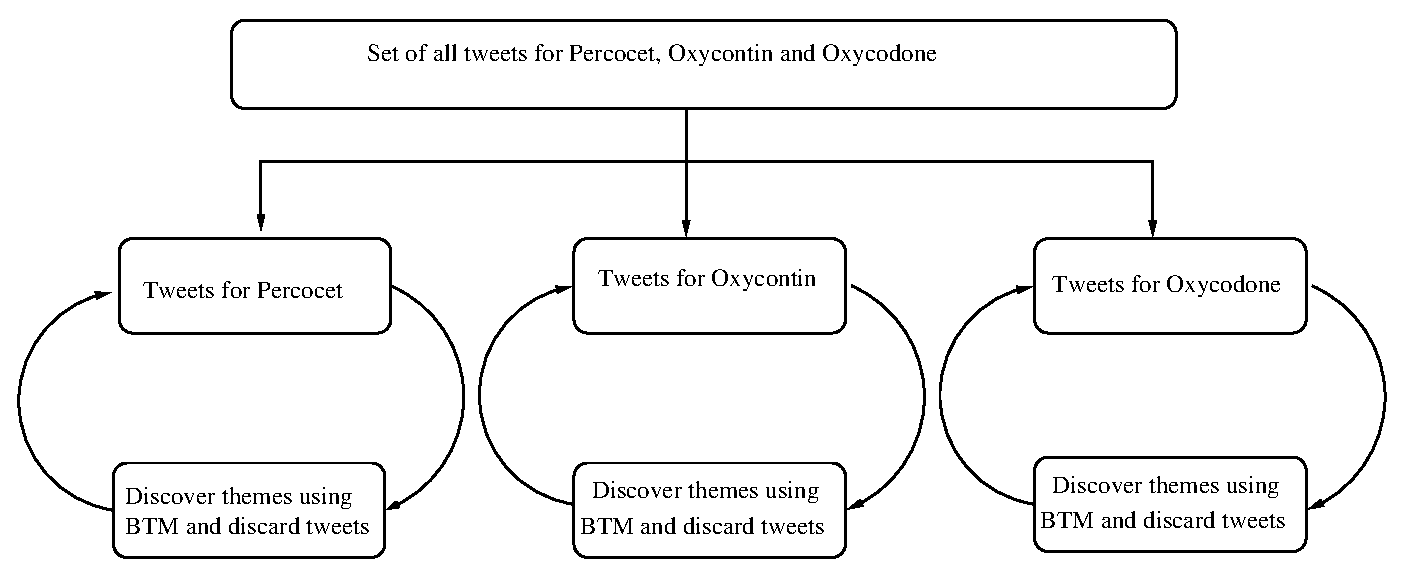
\includegraphics[width=\textwidth]{AB/chart}
\caption[Data analysis overview]{An overview of the steps undertaken in the interative BTM rounds applied to set of all tweets.}
\label{fig:overview_methodology}
\end{figure}

Before the BTM model was applied on the full corpus of 
tweets as described above, the tweets were subjected to 
several standard data preprocessing steps. The first step 
was to produce a subset of tweets corresponding to each drug INN. 
Subsequently, the lang field and the \texttt{user\_lang} field provided 
by the Twitter API were used to remove any non-English tweets. 
From the remaining tweets, all the stopwords were removed. 
For each drug category, a list of vocabulary and the corresponding 
counts were built. Word tokens that occurred less than 
10 times in the corpus of that particular drug were removed 
from all tweets to prevent the model from fitting to what 
could be noisy outliers. Only alphanumeric strings were 
retained, any string with special characters was discarded. 
In addition, any tweet with two or less words was also 
discarded given limited interpretability.

\section{Results}
Table 3 illustrates some examples of the themes 
produced by our BTM machine learning protocol for the three 
prescription opioid analgesic drugs during the first round of the 
iteration, along with the filtering decision that was made as to 
whether or not to retain the tweets pertaining to 
this theme in the subsequent rounds.

\begin{table}
\centering
\small
\begin{tabular}{|c|c|c|c|}
\hline
Drug & example 1 & example 2 & example 3 \\
\hline
Percocet & \pbox{20cm}{super, high, best, \\ buy, online, place, offer,\\ compare, quality} & \pbox{20cm}{percocet, xanax, \\ pop, strippers} & \pbox{20cm}{Percocet, liquor, \\ pour, dose, money, \\ weed}\\
\hline
Filtering decision & \pbox{20cm}{Exclude (example of \\ illicit online sale \\ of controlled substances)}&   Include &Include\\
\hline
\hline
OxyContin & \pbox{20cm}{Oxycontin, bottle, \\ cocaine, drug, \\love, wrong} & \pbox{20cm}{Oxycontin, addiction, \\dangerous, abuse} & \pbox{20cm}{Oxycontin, richest,\\ Forbes, list, \\family, newcomer}\\
\hline
Filtering decision & Include & Include & \pbox{20cm}{Exclude \\(example of\\ news/media content)}\\
\hline
\hline
Oxycodone & \pbox{20cm}{Oxycodone, drug, \\approval, fda, \\media, reports  Heroin} & \pbox{20cm}{oxycodone, cocaine, \\appearance, terrifying, \\change}  & \pbox{20cm}{Canada, monopoly, \\rules, oxycodone, drugs}\\
\hline
Filtering decision &\pbox{20cm} {Exclude \\(example of \\ news/media content)}& Include & \pbox{20cm}{Exclude \\(example of \\news/media content)} \\
\hline
\hline
\end{tabular}
\caption[Example themes discovered for each drug]{This table illustrates some of examples of themes 
discovered for each drug, along with the filtering decision made during the first round of iteration.}
\label{table:themes_filtering_decision}
\end{table}
The themes listed in Table \ref{table:themes_filtering_decision} were annotated manually 
according to the inclusion/exclusion rules laid out in Table \ref{table:inclusion_exclusion}. 
For Percocet, the first example contains keywords like ``buy", ``online", ``offer", ``quality", ``compare" etc. 
This suggests that this topic could be highly correlated with 
tweets promoting illicit prescription drug sales through illegal online pharmacies, 
also a recognized public health threat 
\cite{forman2003availability,forman2006availability,mackey2013digital,raine2009availability}.
Hence, this theme does not satisfy the rules of inclusion from Table \ref{table:inclusion_exclusion}, 
though warrants further examination, 
which is currently being undertaken in a separate study. 
In order to validate the application of these inclusion and 
exclusion rules, a list of 1000 tweets most correlated to this 
theme was retrieved and analyzed by a human coder. 
It was observed that 82\% of all the tweets were about sales 
of prescription drugs through online pharmacies. 
This confirms that the majority of the tweets most correlated 
with this theme indeed do not satisfy the requirements for inclusion.
%
For each of the themes marked as ``Exclude" in the OxyContin and Oxycodone category, 
it appears that some of the identified themes are related to news media 
reports but not individual NMUPD user behavior. 
To evaluate this, the top 1000 most correlated tweets from 
each of the themes were analyzed. 25\%–40\% of these tweets were 
retweets of news headlines. Another 40\% of the tweets were repetitions 
of the same news headlines, even though they were not retweets. 
In fact, in this set of 1000 tweets, there were only a handful of 
unique tweets (ranging between 4–25), most of which were news items. 
Importantly, by eliminating these tweets from subsequent BTM rounds, 
content that is not useful in inferring specific NMUPD behavior 
from individual users can be filtered out in the iterative machine 
learning process applied to a large set of data. 
These analyses also suggest that the top words discovered by 
BTM are indicative of whether or not the theme, and the tweets 
correlated to it, need to be included in the 
subsequent iterations of filtering.

In Table \ref{table:iteration_tweetcounts}, the percentage of tweets retained between 
the first and the second rounds based on our inclusion and 
exclusion criteria was 24\%–36\% (for all three drugs). 
The percentage of tweets retained between the second and 
the third rounds is 72\%–84\%. This increase in the percentage 
of tweets that satisfy the inclusion criteria indicates 
that better NMUPD content saturation is achieved with each round of iteration.

\begin{table}
\begin{tabular}{|c|c|c|c|}
\hline
INN & \#-tweets (or) 1st round & \pbox{20cm}{\% of tweets \\retained for 2nd round \\(from the 1st round)}& \pbox{20cm}{\% of tweets \\retained for 3rd round \\(from the second round)} \\
\hline
Percocet &  5,983,497  & 24\% &84\%\\
OxyContin® & 2,812,364 &  36\% &72\% \\
Oxycodone  & 1,806,900 &  29\% &74\% \\
\hline
\end{tabular}
\caption[Summary of \# of tweets in each round]{This table summarizes the number of tweets used in the first round of iteration, 
and the \% of tweets used in the subsequent rounds.}
\label{table:iteration_tweetcounts}
\end{table}

Table \ref{table:theme_examples_final} illustrates the 
top words from some of the topics obtained after the 
final round of data pruning. All the themes satisfy rules for inclusion 
that were prespecified in Table \ref{table:inclusion_exclusion} suggesting that 
as per the rules, we might have attained saturation. Also, provided in Table 
\ref{table:tweet_examples} are some specific examples of tweets 
randomly sampled from the data after the final round of pruning. 
It is clear that all the tweet examples are related to at 
least one of the themes from Table \ref{table:themes_examples_final}.
In addition, the content of the tweets itself is indicative of NMUPD behavior and abuse.

\begin{table}
\begin{tabular}{|c|c|c|c|}
\hline
Drug & Theme example 1 & Theme example 2 & Theme example 3 \\
\hline
Percocet & \pbox{20cm}{Percocet, addict, \\taking, relax, xanax} & \pbox{20cm}{Percocet, ecstasy, \\adderall, sleep}&\pbox{20cm}{ Percocet,\\ vicodin, gum, \\ball, machine, withdrawal}\\
\hline
OxyContin &  \pbox{20cm}{Oxycontin, pain,\\ addicted, pills} &  \pbox{20cm}{Oxycontin, dangerous, \\abuse, bottle, \\selling, history} & \pbox{20cm}{Oxycontin, niggas, \\roxies, droppin, \\pistols}\\
\hline
Oxycodone& \pbox{20cm}{Oxycodone, ecstasy, \\pain, hugs, \\kisses, xanax}& \pbox{20cm}{Oxycodone, heroin,\\ morphine, addiction,\\ make} &  \pbox{20cm}{Oxycodone, ecstasy, \\pain, xanax}\\
\hline
\end{tabular}
\caption[Example themes after final iteration]{This table illustrates some of examples of themes discovered for each drug after the final iteration of data pruning.}
\label{table:theme_examples_final}
\end{table}
\begin{table}
\begin{tabular}{|c|}
\hline
Example tweets for Percocet: \\
\hline
1. popping percocet and xannies like they some tylenol \\
2. its only 3 pm and ive had a beer and 4 percocets your move bad decisions \\
3. just when i thought that id rock the mic again my brain was fucked up on percocet and vicodine \\
4. i got xanex percocet promethazine with codeine \\
\hline
Example tweets for OxyContin: \\
\hline
1. \pbox{20cm}{i fell in love with a trap mami \\
            she be snortin cocaine and molly sometimes she be \\poppin oxycontin blue pill she be smokin them roxis} \\
2. daydreams laced with oxycontin mind elsewhere \\
3. my mom is ritalin my dad is oxycontin \\
4. i need the zans and oxycontin christ every 2 hours \\
\hline
Example tweets for Oxycodone: \\
\hline
1. \pbox{20cm}{i sure wish i had a \\few beers and maybe \\an oxycodone to make this \\afterglow even more pleasurable}\\
2. \pbox{20cm}{w00t oxycodone and \\morphine i feel like lindsay lohan}\\
3. \pbox{20cm}{that moment when you realize \\the weeknds trademark xo stands for \\ecstacy and oxycodone hence xo \\til we overdose} \\
4. high on coke and oxycodone marijuana is too weak4meh\\
\hline
\end{tabular}
\caption[Spefic examples of tweets after final round]{Randomly sampled examples of tweets obtained from the data after the final round of pruning.}
\label{table:tweet_examples}
\end{table}
In Table \ref{table:theme_examples_final}, almost all of the 
themes mention more than one prescription drug, and in some cases mention 
the use of other illicit drugs (e.g. heroin, ecstasy). 
This suggests that Twitter prescription opioid analgesic abuse content 
and user behavior is highly associated with self-reporting of other forms 
of substance abuse, specific to certain classes of drugs. 
In particular, for the first theme under Percocet, the top words 
suggest that abusing Percocet® and Xanax® is relaxing and addictive. 
While analyzing the top 100 tweets most correlated to this theme, 89\% 
of the tweets were found to be pertinent to the proposed summary. 
In addition, in all three themes for Percocet, different polydrug 
combinations are mentioned with different accompanying adjectives, 
suggesting that each polydrug combination might exhibit its 
own unique form of user described behavior or effect. 
Examining specific examples of tweets identified as highly 
correlated to themes and reproduced in Table \ref{table:tweet_examples} 
further substantiates this pattern. For example, tweets for Percocet 
primarily report use of other prescription drugs 
(examples \#1 and \#4 mention benzodiazepines though example \#2 includes use of alcohol), 
the OxyContin tweets describe various use both 
self-report and observational, and Oxycodone tweets also 
describe poly-use with other illicit drugs.
%
Another likely sign of user initiated and self-reported NMUPD 
behavior is the detection of street or slang terms associated 
with polydrug abuse combinations or drug abuse related behavior. 
This includes the term ``hugs" and ``kisses" in the first theme of 
Oxycodone, both words which used in combination are slang for 
the drug combination of ecstasy and oxycodone, which are also 
keywords included in the theme (Table \ref{table:tweet_examples}, example \#2 under 
Oxycodone). Similarly, the term ``roxies" are included in the OxyContin second theme, 
which is a slang term for Roxicodone, another opioid analgesic (oxycodone hydrochloride). 
Table \ref{table:tweet_examples} also contains other controlled 
substances like Ritalin, Prednisone, Valium and Marijuana.
%
In order to assess the quality of themes that emerged after the 
final round of data pruning two types of evaluations were performed. 
The first was a supervised evaluation that involved manually annotating 
the tweets from each theme as being relevant or irrelevant to the theme detected. 
From each theme, a maximum of 2000 most correlated tweets were retrieved and annotated. 
The average false positive rate was calculated across all the themes for each drug. 
While manually annotating tweets for their relevance to NMUPD behavior, 
it was observed that the dataset contained several retweets. So, even if one tweet 
was found to be irrelevant, it was often the case that the tweet was 
retweeted several times; thereby increasing the false positive rate. 
In addition, there were also scenarios where even though a tweet contained 
keywords indicating polydrug abuse and/or potential adverse effects, 
the intent of the tweet remained vague. Such tweets were also marked as 
irrelevant during manual annotation. The results of the total number of 
tweets after the final round of machine learning, and the 
false positive rate for each drug is summarized in Table 7.
%
\begin{table}
\begin{tabular}{|c|c|c|c|c|}
\hline
Drug &   \#-tweets &   \pbox{20cm}{Average FP-rate} & \pbox{20cm}{Average cluster \\purity across \\themes}&\pbox{20cm}{Purity of \\a set of random tweets}\\
\hline
Percocet &   1,231,641  & 55\% &0.4348 & 0.2378\\
Oxycontin &  741,272 &28\% &0.5678&  0.2219\\
Oxycodone  & 380,838& 14\%& 0.6729 & 0.1976\\
\hline
\end{tabular}
\caption[Evaluation of themes]{Summary of results of evaluating the quality of the themes obtained after the final round of data pruning.}
\label{table:evaluating_themes}
\end{table}
The second was an unsupervised evaluation that involved the 
calculation of a metric called cluster purity \cite{Bishop_2006}. 
This metric quantifies how coherent a theme is. If the tweets 
belonging to a theme are very diverse in terms of their content, 
that theme is considered incoherent, and the resulting 
purity score will be low; and vice versa. In order to obtain 
the cluster purity score for each theme, we considered the same 
2000 most correlated tweets as before and calculated the average 
similarity between all pairs of tweets from this set.
This average similarity is the cluster purity of the theme. 
As baseline, we randomly sampled 2000 tweets from our original 
dataset of 11 M tweets, and calculated the average similarity 
between all pairs from this random set. The results are summarized 
in the last two columns of Table \ref{table:evaluating_themes}. 
The cluster purity for each drug is up to 3 times better than 
that of a random set of tweets. Both the supervised and unsupervised 
evaluations suggest that the themes obtained after the 
final round of data pruning are of good quality.
%
\section{Conclusion}
In summary, the results of this study suggest that the use 
of an automated methodology that employs iterative rounds of 
unassisted machine learning has the potential to filter and 
analyze large and complex social media conversational datasets 
with minimal human intervention such as through the use of 
manual content analysis or human annotation. 
Importantly, the study also demonstrates that a machine 
learning algorithm, such as the one employed in this study, 
can be used to identify themes in NMUPD use and behavior that 
are important in identifying macro and emerging trends in the 
context of broader prescription opioid analgesic abuse behavior.
%
Primarily, in this study, the central theme that emerged was 
that polydrug abuse is predominantly associated with Twitter 
prescription drug abuse discussions and could be indicative 
of larger behavioral trends of users abusing multiple prescription 
drugs and also combining use with other illicit substances. 
These results could form the basis for future in-depth studies 
examining the unique health and substance abuse consequences 
associated highly prevalent polydrug uses (including potentially 
linkages to mental health issues and behavior among young adults 
and adolescents already identified in the literature)
\cite{mackesy2015prescription,kelly2014combinations,fink2015patterns}. 

The study is also important within the context of future research 
attempting to effectively scale projects for big data analyses. 
Primarily, the methodology allows for the machine learning processes to ``pre-filter" 
millions of Tweets, better isolating content that is highly relevant to 
a research question (such as prescription opioid analgesic abuse) based upon a 
researcher's own desired set of inclusion/exclusion criteria drawn from 
behavioral risk factors identified in the literature or through traditional 
survey instruments. Following this process of machine driven filtering, 
a smaller subset of tweets/content can be identified for more 
in-depth analysis and confirmation by human coders to better assess 
the accuracy of identified themes to highly correlated content. 
Overall, the methodology represents an innovative approach that has 
the advantages of reliably identifying themes of interest from 
large amounts of data collected at a point of time from the 
Twitter public API.
%
\subsection{Limitations}
%
One of our primary aims in this study was to increase the 
signal to noise ratio in the tweets that contain the three 
NMUPD keywords so that the filtered dataset contains only 
those messages which are relevant to NMUPD usage and behavior. 
Certain aspects of our methodology have inherent limitations in 
achieving this goal. Firstly, we faced scenarios where the text of the 
tweet would satisfy all the inclusion criteria (hence the theme 
detected from this tweet, and similar ones might be marked for 
inclusion in subsequent iterative rounds of filtering), but 
the intent of the tweet remained vague (e.g. due to its 
brevity or lack of sufficient description). Hence, while human 
coders reviewing a sample of tweets would likely mark such tweets 
as being not relevant, such tweets (and the themes they 
belonged to), inadvertently increase the false positive rate. 
Several tweets contained hyperlinks, the content of which might 
have helped to better contextualize the original tweets; 
especially those with vague intents. However, this study primarily 
considered only the text of the tweets, and did not conduct 
further analysis into the content of hyperlinks, which in past 
studies have been identified as containing pictures, videos 
and other media confirming drug abuse behavior \cite{katsuki2015establishing}. 
The second aim was to identify themes about NMUPD usage and behavior 
in the Twittersphere. This study is more of an exploratory study that 
attempts to determine the major themes prevalent on Twittersphere when 
it comes to opioid analgesic NMUPD. However, in order to gain a full 
understanding, crowdsourced or large scale human coding of data 
augmented by a cohort of NMUPD users to corroborate findings would 
be the optimal methodology for future consideration. Lastly, a non-trivial 
amount of content on Twitter contains special characters that do not 
fall under the alphanumeric character categorization. Hence, by 
ommitting content that is not alphanumeric, we might inadvertently 
be discarding some useful information.
%
\subsection{Future directions}
%
The data spans a period of 6 months (June to November 2015). 
However, for the purposes of this study, the timestamps of the tweet were not taken into account during the learning process.
%
Future studies could attempt to identify changes in 
NMUPD behavioral trends and attitudes over time through a longitudinal 
study design. We also observed that a significant number of 
themes that are attributable to the possible sale of controlled 
substances by illicit online pharmacies. Future studies should 
specifically examine this potential pathway for illicit prescription 
drug access and its negative impact on NMUPD behavior, dependence, and addiction.
